\documentclass[compress,aspectratio=169]{beamer}
\usepackage{irbookslide}
\usepackage{irilmenau2}
\usepackage{tikz}
\usetikzlibrary{shapes}
\usepackage{url}
\usepackage{ifxetex}
%\RequireXeTeX
\usepackage{fontspec} % zahteva paket euenc
\usepackage{xunicode}
\usepackage{xltxtra}
\usepackage{polyglossia}
\usepackage{minted}
\usepackage[noend]{algorithmic}
\renewcommand{\algorithmicrequire}{\textbf{Input:}}
\renewcommand{\algorithmicensure}{\textbf{Output:}}
\renewcommand{\algorithmiccomment}[1]{\hfill \{\myred{#1}\}}
\usepackage{xcolor,colortbl}
\usepackage{textcomp}
\usepackage{unicode-math}
%\usepackage{hyphenat}
%\setdefaultlanguage[script=Latin]{serbian}

\title{Stabla pretrage}
\author{\textcopyright \ \ Goodrich, Tamassia, Goldwasser}
\institute{Katedra za informatiku, Fakultet tehničkih nauka, Univerzitet u
Novom Sadu}
\date{2021.}
\subject{Predavanja sa ASP}

\begin{document}

\frame{\titlepage}

\section[Binarno stablo]{Binarno stablo pretrage}
\begin{frame}[fragile]
  \frametitle{Mape sa poretkom}
  \begin{itemize}
    \item postoji relacija poretka nad ključevima 
    \item elementi se skladište prema vrednosti ključa
    \item pretrage ,,najbliži sused`` (nearest neighbor):
    \begin{itemize}
      \item nađi element sa najvećim ključem manjim ili jednakim $k$
      \item nađi element sa najmanjim ključem većim ili jednakim $k$
    \end{itemize}
  \end{itemize}
\end{frame}

\begin{frame}[fragile]
  \frametitle{Binarna pretraga}
  \begin{itemize}
    \item binarna pretraga može da pronađe ,,najbližeg suseda`` za mapu sa poretkom implementiranu pomoću niza koji je sortiran po ključu 
    \begin{itemize}
      \item u svakom koraku prepolovi se broj kandidata
      \item radi u $O(\log n)$ vremenu
    \end{itemize}
    \item primer: nađi 7 
  \end{itemize}
  \begin{center}
    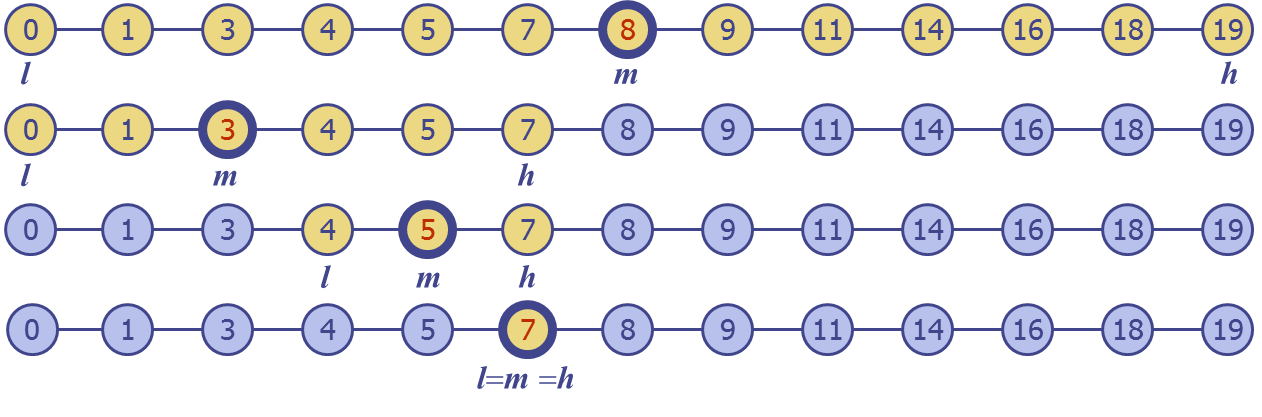
\includegraphics[width=10cm]{asp-11-pic01.png}
  \end{center}
\end{frame}

\begin{frame}[fragile]
  \frametitle{Tabela pretrage}
  \begin{itemize}
    \item tabela pretrage je mapa sa poretkom implementirana pomoću sortiranog niza 
    \begin{itemize}
      \item eksterni komparator za ključeve
    \end{itemize}
    \item performanse: 
    \begin{itemize}
      \item binarna pretraga je $O(\log n)$
      \item dodavanje je $O(n)$
      \item uklanjanje je $O(n)$
    \end{itemize}
    \item radi efikasno samo za mali broj elemenata ili tamo gde je pretraga česta a izmene retke (npr. provera kreditne kartice) 
  \end{itemize}
\end{frame}

\begin{frame}[fragile]
  \frametitle{Sortirana mapa ATP}
  \begin{itemize}
    \item standardne operacije mape 
  \end{itemize}
  \begin{center}
    \begin{tabular}{rp{8cm}}
      \textbf{\texttt{M[k]}} & vraća vrednost $v$ za ključ $k$ u mapi $M$; implementira je \texttt{\_\_getitem\_\_} \\ \hline
      \textbf{\texttt{M[k]=v}} & dodaje novi element $(k, v)$ u $M$ ili menja postojeći; implementira je \texttt{\_\_setitem\_\_} \\ \hline
      \textbf{\texttt{del M[k]}} & uklanja element sa ključem $k$ iz $M$; implementira je \texttt{\_\_delitem\_\_} \\
    \end{tabular}
  \end{center}
  \begin{itemize}
    \item dodatne funkcionalnosti 
    \begin{itemize}
      \item sortiran redosled prilikom iteracije
      \item nađi veće: \myred{find\_gt}($k$)
      \item nađi u opsegu: \myred{find\_range}($start, stop$) 
    \end{itemize}
  \end{itemize}
\end{frame}

\begin{frame}[fragile]
  \frametitle{Binarno stablo pretrage}
  \begin{itemize}
    \item \myred{binarno stablo pretrage} je binarno stablo koje čuva $(k, v)$ parove u čvorovima $p$ tako da važi:
    \begin{itemize}
      \item ključevi koji se nalaze u \textbf{levom} podstablu od $p$ su \textbf{manji} od $k$
      \item ključevi koji se nalaze u \textbf{desnom} podstablu od $p$ su \textbf{veći} od $k$
    \end{itemize}
    \item listovi ne čuvaju elemente, reference na listove mogu biti None
    \item inorder obilazak: ključevi u rastućem redosledu 
  \end{itemize}
  \begin{center}
    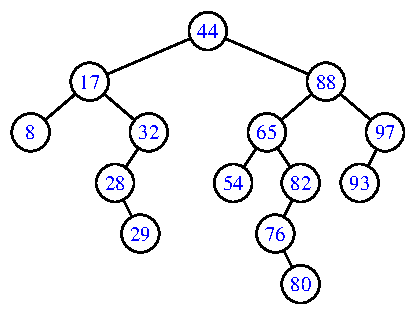
\includegraphics[width=5.5cm]{asp-11-pic02.pdf}
  \end{center}
\end{frame}

\begin{frame}[fragile]
  \frametitle{Pretraga u binarnom stablu}
  \begin{itemize}
    \item tražimo ključ $k$ polazeći od korena
    \item idemo levo ako je $k$ manji od tekućeg čvora
    \item idemo desno ako je $k$ veći od tekućeg čvora
    \item ako dođemo do lista, $k$ nije nađen
  \end{itemize}
  \begin{columns}
    \begin{column}[c]{6cm}
      \begin{center}
        Tražimo 65
        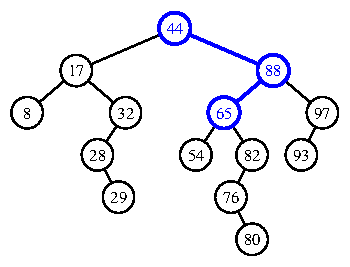
\includegraphics[width=5.8cm]{asp-11-pic03a.pdf}
      \end{center}
    \end{column}  
    \begin{column}[c]{6cm}
      \begin{center}
        Tražimo 68
        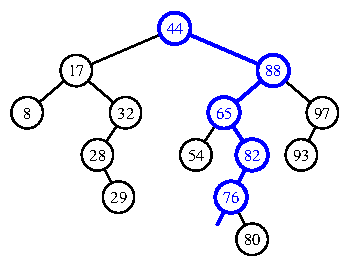
\includegraphics[width=5.8cm]{asp-11-pic03b.pdf}
      \end{center}
    \end{column}  
  \end{columns}
\end{frame}

\renewcommand{\algorithmiccomment}[1]{\hfill \{\myred{#1}\}}

\begin{frame}[fragile]
  \frametitle{Pretraga u binarnom stablu}
\myred{TreeSearch}($T, p, k$)
\begin{algorithmic}
\IF{$k = p.key$}
  \RETURN $p$ \COMMENT{pronađen}
\ELSIF{$k < p.key \land T.left(p) \neq None$}
  \RETURN TreeSearch($T, T.left(p), k$) \COMMENT{levo podstablo}
\ELSIF{$k > p.key \land T.right(p) \neq None$}
  \RETURN TreeSearch($T, T.right(p), k$) \COMMENT{desno podstablo}
\ENDIF
\RETURN None  \COMMENT{nije pronađen}
\end{algorithmic}
\end{frame}

\begin{frame}[fragile]
  \frametitle{Performanse pretrage u binarnom stablu}
  \begin{itemize}
    \item u svakom rekurzivnom pozivu spuštamo se za jedan nivo u stablu
    \item testiranje u okviru jednog nivoa je $O(1)$
    \item ukupan broj testova je $O(h)$, gde je $h$ visina stabla
  \end{itemize}
  \begin{center}
    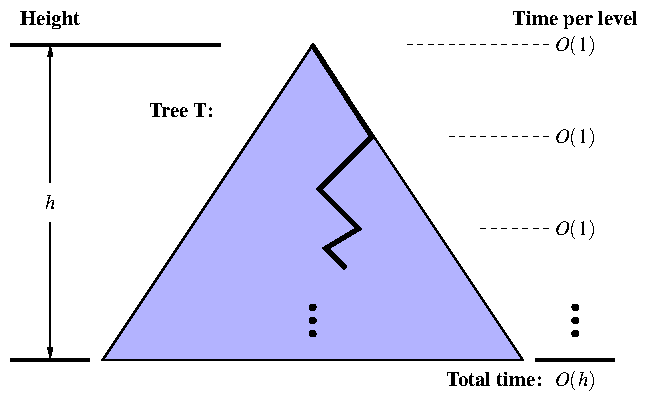
\includegraphics[width=8cm]{asp-11-pic04.pdf}
  \end{center}
\end{frame}

\begin{frame}[fragile]
  \frametitle{Dodavanje u stablo}
  \begin{itemize}
    \item dodajemo element $(k, v)$
    \item prvo tražimo $k$
    \item ako $k$ nije u stablu, došli smo do lista gde treba dodati čvor
    \item primer: dodajemo 68
  \end{itemize}
  \begin{columns}
    \begin{column}[c]{6cm}
      \begin{center}
        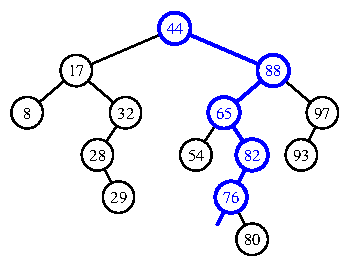
\includegraphics[width=6cm]{asp-11-pic05a.pdf}
      \end{center}
    \end{column}  
    \begin{column}[c]{6cm}
      \begin{center}
        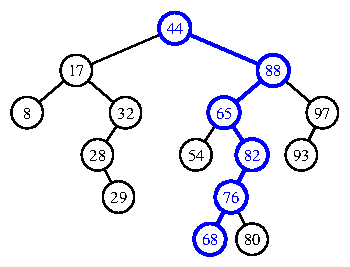
\includegraphics[width=6cm]{asp-11-pic05b.pdf}
      \end{center}
    \end{column}  
  \end{columns}
\end{frame}

\begin{frame}[fragile]
  \frametitle{Dodavanje u stablo}
\myred{TreeInsert}($T, k, v$)
\begin{algorithmic}
\STATE $p \leftarrow$ TreeSearch($T, T.root, k$)
\IF{$k = p.key$}
  \STATE $p.value \leftarrow v$  \COMMENT{ako već postoji zameni vrednost}
\ELSIF{$k < p.key$}
  \STATE $p$.add\_left($k, v$) \COMMENT{dodaj levo dete}
\ELSE
  \STATE $p$.add\_right($k, v$) \COMMENT{dodaj desno dete}
\ENDIF
\end{algorithmic}
  \begin{itemize}
    \item dodaje se uvek u list
  \end{itemize}
\end{frame}

\begin{frame}[fragile]
  \frametitle{Uklanjanje iz stabla}
  \begin{itemize}
    \item uklanjamo element sa ključem $k$
    \item prvo nađemo $p$ koji sadrži $k$
    \item ako $p$ ima \textbf{najviše jedno} dete
    \item njegovo dete $r$ vežemo u stablo umesto njega
    \item primer: uklanjamo 32
  \end{itemize}
  \begin{columns}
    \begin{column}[c]{6cm}
      \begin{center}
        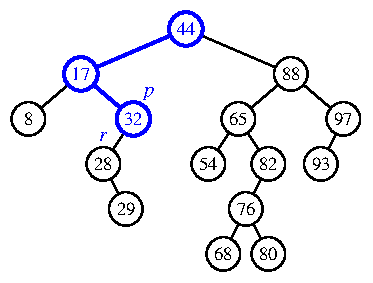
\includegraphics[width=5.8cm]{asp-11-pic06a.pdf}
      \end{center}
    \end{column}  
    \begin{column}[c]{6cm}
      \begin{center}
        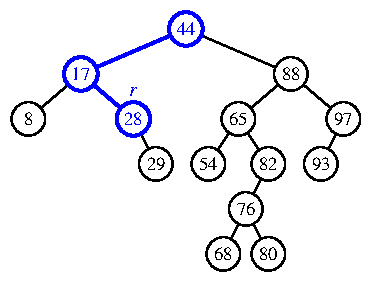
\includegraphics[width=5.8cm]{asp-11-pic06b.pdf}
      \end{center}
    \end{column}  
  \end{columns}
\end{frame}

\begin{frame}[fragile]
  \frametitle{Uklanjanje iz stabla}
  \begin{itemize}
    \item ako $p$ ima \textbf{dva} deteta
    \begin{itemize}
      \item nađemo čvor $r$ čiji ključ neposredno prethodi $p$ -- to je ,,najdesniji`` čvor u njegovom levom podstablu
      \item vežemo $r$ na mesto $p$; pošto $r$ neposredno prethodi $p$ po vrednosti ključa, svi elementi u desnom podstablu od $p$ su veći od $r$ i svi elementi u levom podstablu od $p$ su manji od $r$
      \item treba još obrisati stari $r$ -- pošto je to ,,najdesniji`` element, on nema desno dete, pa se može obrisati po prethodnom algoritmu
    \end{itemize}
  \end{itemize}
\end{frame}

\begin{frame}[fragile]
  \frametitle{Uklanjanje iz stabla}
  \begin{itemize}
    \item ako $p$ ima \textbf{dva} deteta
    \item primer: uklanjamo 88
  \end{itemize}
  \begin{columns}
    \begin{column}[c]{6cm}
      \begin{center}
        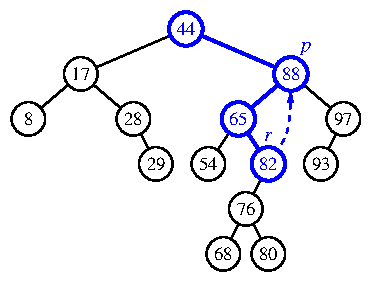
\includegraphics[width=6cm]{asp-11-pic07a.pdf}
      \end{center}
    \end{column}  
    \begin{column}[c]{6cm}
      \begin{center}
        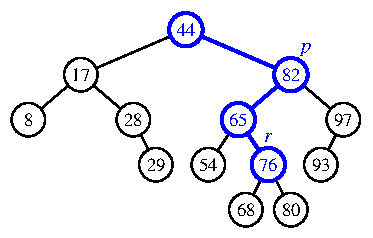
\includegraphics[width=6cm]{asp-11-pic07b.pdf}
      \end{center}
    \end{column}  
  \end{columns}
\end{frame}

\begin{frame}[fragile]
  \frametitle{Performanse binarnog stabla pretrage}
  \begin{columns}
    \begin{column}[c]{6cm}
      \begin{itemize}
        \item zauzeće memorije je $O(n)$
        \item pretraga, dodavanje i uklanjanje su $O(h)$
        \item visina stabla $h$ je $O(\log n) \leq h \leq O(n)$
      \end{itemize}
    \end{column}  
    \begin{column}[c]{6cm}
      \begin{center}
        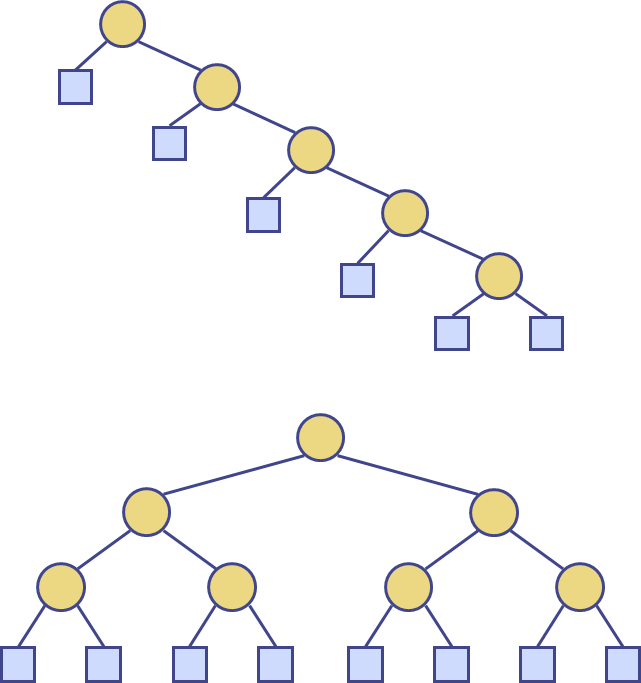
\includegraphics[width=5cm]{asp-11-pic08.png}
      \end{center}
    \end{column}  
  \end{columns}
  \ \\ \hfill balansirano stablo ima bolje performanse
\end{frame}

\section[Balansiranje]{Balansiranje binarnog stabla}
\begin{frame}[fragile]
  \frametitle{Balansiranje binarnog stabla}
  \begin{itemize}
    \item osnovna operacija za balansiranje je \myred{rotacija}
    \item ,,rotiramo`` dete i njegovog roditelja
    \item tom prilikom i podstabla menjaju mesta
    \item jedna rotacija traje $O(1)$
  \end{itemize}
  \begin{center}
    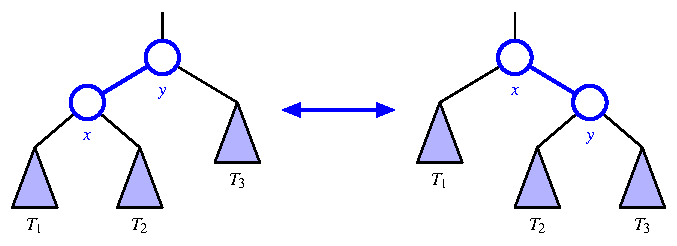
\includegraphics[width=10cm]{asp-11-pic09.pdf}
  \end{center}
\end{frame}

\begin{frame}[fragile]
  \frametitle{Balansiranje binarnog stabla}
  \begin{itemize}
    \item kompozitna operacija ,,\myred{restrukturiranje tri čvora}`` (tri-node restructuring)
    \item posmatraju se čvor, njegovo dete i unuče
    \item cilj je da se skrati putanja od čvora do unučeta
    \item četiri moguća rasporeda čvorova
    \begin{itemize}
      \item prva dva traže jednu rotaaciju
      \item druga dva traže dve rotacije
    \end{itemize}
  \end{itemize}
\end{frame}

\begin{frame}[fragile]
  \frametitle{Restrukturiranje sa jednom rotacijom}
  \begin{center}
    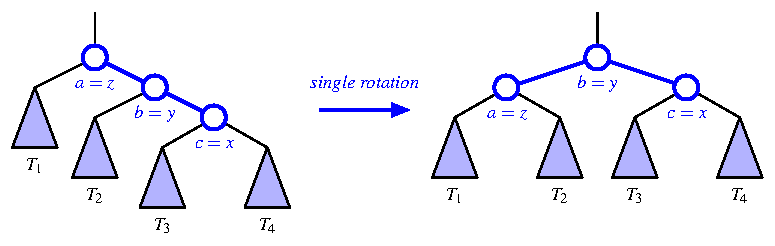
\includegraphics[width=10cm]{asp-11-pic10.pdf}
  \end{center}
  \begin{center}
    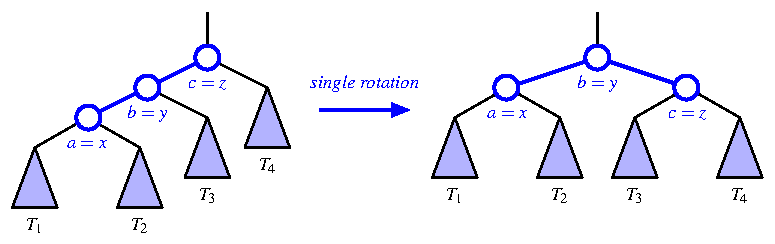
\includegraphics[width=10cm]{asp-11-pic11.pdf}
  \end{center}
\end{frame}

\begin{frame}[fragile]
  \frametitle{Restrukturiranje sa dve rotacije}
  \begin{center}
    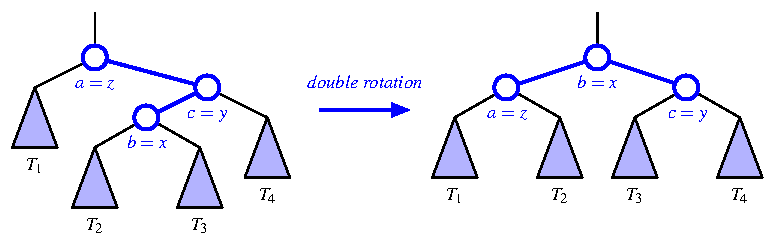
\includegraphics[width=10cm]{asp-11-pic12.pdf}
  \end{center}
  \begin{center}
    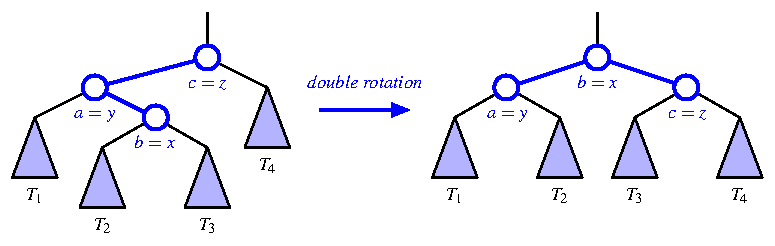
\includegraphics[width=10cm]{asp-11-pic13.pdf}
  \end{center}
\end{frame}

\section[AVL stablo]{AVL stablo}

\begin{frame}[fragile]
  \frametitle{AVL stablo}
  \begin{itemize}
    \item autori: G.M. \myred{A}delson-\myred{V}elskii i E. \myred{L}andis
    \item visina podstabla: broj čvorova na najdužoj putanji od korena do lista
    \item visina čvora = visina podstabla sa njim kao korenom
    \item \myred{AVL stablo} je binarno stablo koje ima dodatnu osobinu:
    \begin{itemize}
      \item za svaki čvor u stablu, visine njegove dece razlikuju se najviše za 1
    \end{itemize}
  \end{itemize}
  \begin{center}
    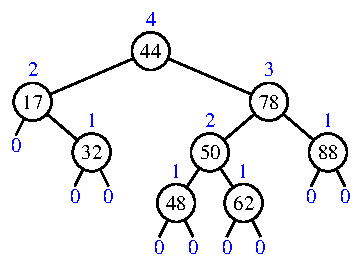
\includegraphics[width=5cm]{asp-11-pic14.pdf}
  \end{center}
\end{frame}

\begin{frame}[fragile]
  \frametitle{Visina AVL stabla}
  \begin{itemize}
    \item \textbf{teorema}: visina AVL stabla sa $n$ čvorova je $O(\log n)$
    \item \textbf{dokaz}: $n(h)$ -- najmanji broj unutrašnjih čvorova u AVL stablu visine $h$
    \item očevidno: $n(1)=1$, $n(2)=2$
    \item za $n>2$, AVL stablo visine $h$ sadrži koren, podstablo visine $h-1$ i podstablo visine $h-2$
    \item tj. $n(h) = 1 + n(h-1) + n(h-2)$
    \item kako je $n(h-1)>n(h-2)$, važi $n(h)>2n(h-2)$
    \begin{itemize}
      \item indukcijom: $n(h)>2n(h-2)$, $n(h)>4n(h-4)$, $n(h)>8(h-6)$, \ldots
      \item \myred{$n(h)>2^in(h-2i)$}
    \end{itemize}
    \item bazni slučaj: $n(h)>2^{h/2-1}$
    \item odnosno: $h < 2\log n(h) + 2$
    \item tj. visina AVL stabla $h$ je $O(\log n)$
  \end{itemize}
\end{frame}

\begin{frame}[fragile]
  \frametitle{AVL stablo: dodavanje}
  \begin{itemize}
    \item stablo u koje dodajemo novi čvor je AVL stablo
    \item dodavanje se vrši isto kao kod binarnog stabla -- u list
    \item dodavanje može da naruši balansiranost
    \item čvorovi koji mogu biti disbalansirani su samo preci novog čvora
    \item primer: dodajemo čvor 54
  \end{itemize}
  \begin{columns}
    \begin{column}[t]{6cm}
        pre balansiranja 
        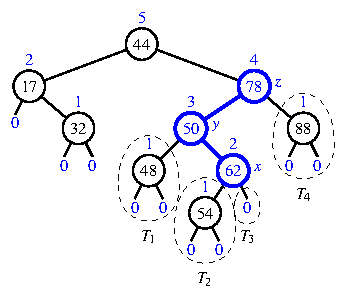
\includegraphics[width=5cm]{asp-11-pic15a.pdf}
    \end{column}  
    \begin{column}[t]{6cm}
        posle balansiranja
        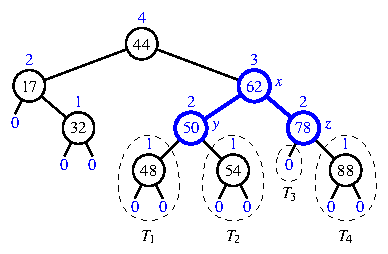
\includegraphics[width=6cm]{asp-11-pic15b.pdf}
    \end{column}  
  \end{columns}
\end{frame}

\begin{frame}[fragile]
  \frametitle{AVL stablo: dodavanje}
  \begin{itemize}
    \item ,,search-and-repair`` strategija
    \item $z$ -- prvi nebalansirani čvor na polazeći od $p$ koji smo naišli
    %\item $y$ -- dete $z$ sa većom visinom (takođe predak $p$)
    %\item $y$ -- dete $y$ sa većom visinom (predak $p$ ili sâm $p$)
    \item radimo \textbf{trinode restructuring} za $z$ 
  \end{itemize}
  \begin{columns}
    \begin{column}[t]{6cm}
      \begin{center}
        pre balansiranja 
        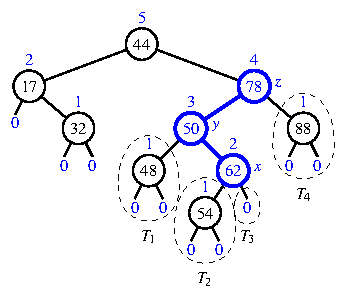
\includegraphics[width=5cm]{asp-11-pic15a.pdf}
      \end{center}
    \end{column}  
    \begin{column}[t]{6cm}
      \begin{center}
        posle balansiranja
        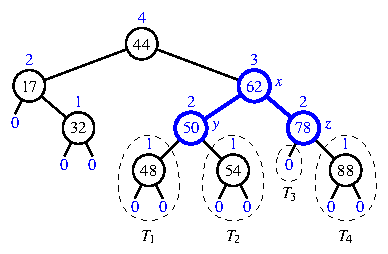
\includegraphics[width=6cm]{asp-11-pic15b.pdf}
      \end{center}
    \end{column}  
  \end{columns}
\end{frame}

\begin{frame}[fragile]
  \frametitle{AVL stablo: dodavanje}
pre dodavanja: 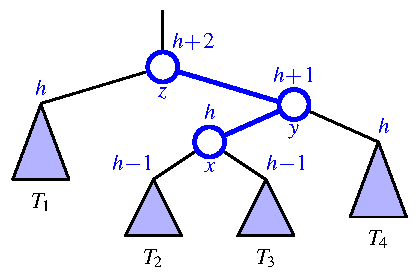
\includegraphics[width=3.5cm]{asp-11-pic16a.pdf}

dodavanje u $T_3$ remeti balans u $z$: 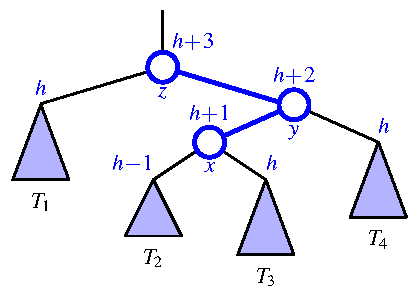
\includegraphics[width=3.5cm]{asp-11-pic16b.pdf}

nakon restrukturiranja: 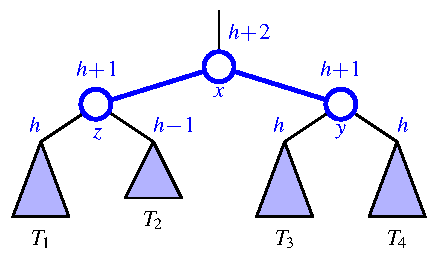
\includegraphics[width=3.5cm]{asp-11-pic16c.pdf}
\end{frame}

\begin{frame}[fragile]
  \frametitle{AVL stablo: uklanjanje}
  \begin{itemize}
    \item uklanjanjem se može narušiti balans AVL stabla
    \item i ovde radimo restrukturiranje posle uklanjanja
    \item primer: uklanjamo 32
  \end{itemize}
  \begin{columns}
    \begin{column}[t]{6cm}
      \begin{center}
        pre balansiranja, koren nije balansiran 
        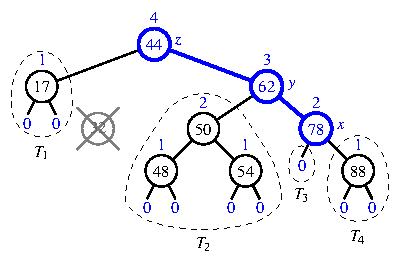
\includegraphics[width=5cm]{asp-11-pic17a.pdf}
      \end{center}
    \end{column}  
    \begin{column}[t]{6cm}
      \begin{center}
        posle balansiranja (jedna rotacija)
        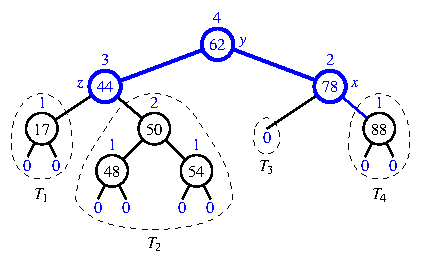
\includegraphics[width=6cm]{asp-11-pic17b.pdf}
      \end{center}
    \end{column}  
  \end{columns}
\end{frame}

\begin{frame}[fragile]
  \frametitle{AVL stablo: performanse}
  \begin{itemize}
    \item jedno restrukturiranje je $O(1)$ 
    \item pretraga je $O(\log n)$ -- visina stabla je $O(\log n)$
    \item dodavanje je $O(\log n)$
    \begin{itemize}
      \item pronalaženje mesta je $O(\log n)$
      \item restrukturiranje uz stablo je $O(\log n)$
    \end{itemize}
    \item uklanjanje je $O(\log n)$
    \begin{itemize}
      \item pronalaženje mesta je $O(\log n)$
      \item restrukturiranje uz stablo je $O(\log n)$
    \end{itemize}
  \end{itemize}
\end{frame}

\section[Splay stablo]{Splay stablo}
\begin{frame}[fragile]
  \frametitle{Splay stablo}
  \begin{itemize}
    \item \myred{splay}: ,,rašireno`` 
    \item ne nameće logaritamsko ograničenje na visinu
    \item \myred{splaying}: ,,širenje`` stabla prilikom dodavanja, uklanjanja \textbf{i pretrage}
    \item ideja: da češće korišćeni elementi budu bliže korenu
  \end{itemize}
\end{frame}

\begin{frame}[fragile]
  \frametitle{Splaying}
  \begin{itemize}
    \item čvor $x$ se premešta u koren nizom restrukturiranja 
    \item operacije restrukturiranja zavise od položaja $x$, $y$ (roditelja) i $z$ (dede, ako postoji)
    \item postoje tri slučaja:
    \begin{itemize}
      \item \myred{zig-zig}
      \item \myred{zig-zag}
      \item \myred{zig}
    \end{itemize}
  \end{itemize}
\end{frame}

\begin{frame}[fragile]
  \frametitle{Splaying: zig-zig}
  \begin{itemize}
    \item $x$ i $y$ su  
    \begin{itemize}
      \item obojica levo dete svog roditelja ili
      \item obojica desno dete svog roditelja
    \end{itemize}
    \item $x$ postaje koren, $y$ njegovo dete, $z$ njegovo unuče
  \end{itemize}
  \begin{columns}
    \begin{column}[t]{6cm}
      \begin{center}
        pre zig-zig 
        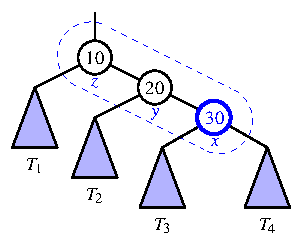
\includegraphics[width=5cm]{asp-11-pic18a.pdf}
      \end{center}
    \end{column}  
    \begin{column}[t]{6cm}
      \begin{center}
        posle zig-zig
        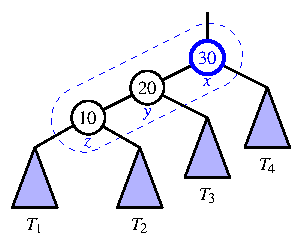
\includegraphics[width=5cm]{asp-11-pic18b.pdf}
      \end{center}
    \end{column}  
  \end{columns}
\end{frame}

\begin{frame}[fragile]
  \frametitle{Splaying: zig-zag}
  \begin{itemize}
    \item $x$ i $y$ 
    \begin{itemize}
      \item prvi je levo dete a drugi je desno dete, ili
      \item prvi je desno dete a drugi je levo dete
    \end{itemize}
    \item $x$ postaje koren, $y$ i $z$ njegova deca
  \end{itemize}
  \begin{columns}
    \begin{column}[t]{6cm}
      \begin{center}
        pre zig-zag 
        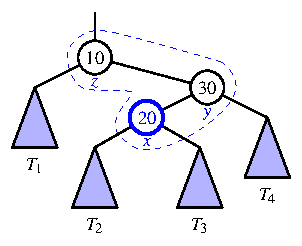
\includegraphics[width=5cm]{asp-11-pic19a.pdf}
      \end{center}
    \end{column}  
    \begin{column}[t]{6cm}
      \begin{center}
        posle zig-zag
        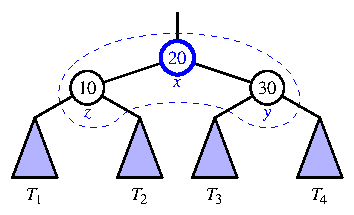
\includegraphics[width=6cm]{asp-11-pic19b.pdf}
      \end{center}
    \end{column}  
  \end{columns}
\end{frame}

\begin{frame}[fragile]
  \frametitle{Splaying: zig}
  \begin{itemize}
    \item $x$ ima roditelja $y$ ali nema dedu $z$ \ \ :(
    \item $x$ postaje koren, $y$ njegovo dete
  \end{itemize}
  \begin{columns}
    \begin{column}[t]{6cm}
      \begin{center}
        pre zig
        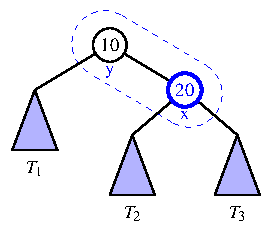
\includegraphics[width=5cm]{asp-11-pic20a.pdf}
      \end{center}
    \end{column}  
    \begin{column}[t]{6cm}
      \begin{center}
        posle zig
        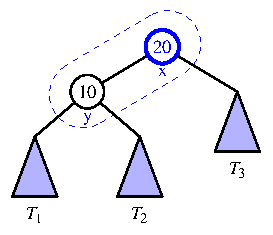
\includegraphics[width=5cm]{asp-11-pic20b.pdf}
      \end{center}
    \end{column}  
  \end{columns}
\end{frame}

\begin{frame}[fragile]
  \frametitle{Splaying: primer $_1$}
  \begin{itemize}
    \item zig-zig, zig-zag i zig primenjujemo sve dok $x$ ne postane koren
    \item primer: dodajemo 14
    \item na 14 se primenjuje zig-zag (jer 14 je desno dete a 13 je levo dete)
  \end{itemize}
  \begin{center}
    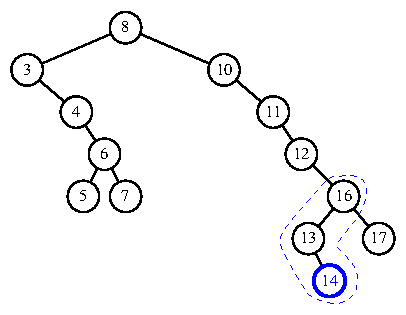
\includegraphics[width=7cm]{asp-11-pic21.pdf}
  \end{center}
\end{frame}

\begin{frame}[fragile]
  \frametitle{Splaying: primer $_2$}
  \begin{itemize}
    \item posle primenjenog zig-zag stanje je
  \end{itemize}
  \begin{center}
    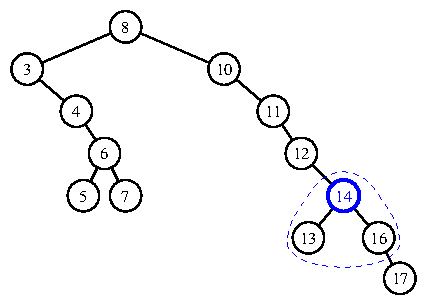
\includegraphics[width=7cm]{asp-11-pic22.pdf}
  \end{center}
\end{frame}

\begin{frame}[fragile]
  \frametitle{Splaying: primer $_3$}
  \begin{itemize}
    \item sada može da se primeni zig-zig
  \end{itemize}
  \begin{center}
    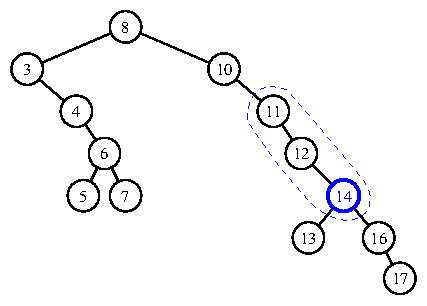
\includegraphics[width=7cm]{asp-11-pic23.pdf}
  \end{center}
\end{frame}

\begin{frame}[fragile]
  \frametitle{Splaying: primer $_4$}
  \begin{itemize}
    \item nakon primene zig-zig
  \end{itemize}
  \begin{center}
    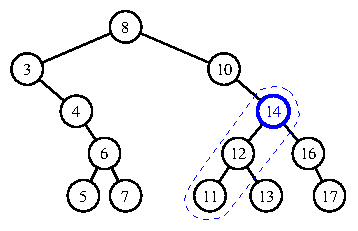
\includegraphics[width=7cm]{asp-11-pic24.pdf}
  \end{center}
\end{frame}

\begin{frame}[fragile]
  \frametitle{Splaying: primer $_5$}
  \begin{itemize}
    \item sada može ponovo zig-zig
  \end{itemize}
  \begin{center}
    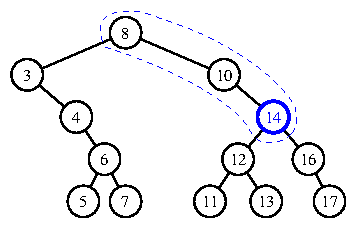
\includegraphics[width=7cm]{asp-11-pic25.pdf}
  \end{center}
\end{frame}

\begin{frame}[fragile]
  \frametitle{Splaying: primer $_6$}
  \begin{itemize}
    \item nakon drugog zig-zig
  \end{itemize}
  \begin{center}
    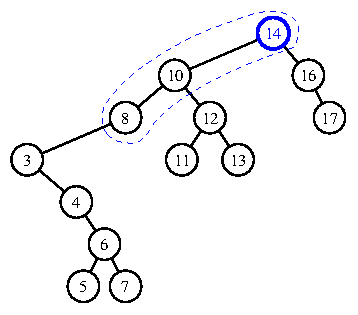
\includegraphics[width=7cm]{asp-11-pic26.pdf}
  \end{center}
\end{frame}

\begin{frame}[fragile]
  \frametitle{Splay stablo: performanse}
  \begin{itemize}
    \item zig-zig, zig-zag i zig su $O(1)$
    \item splaying čvora $p$ je $O(d)$ gde je $d$ dubina čvora $p$
    \item tj. isto koliko je potrebno i za navigaciju od korena do $p$ \\ \ \\
    \item u najgorem slučaju, pretraga, dodavanje i uklanjanje su $O(h)$ gde je $h$ visina stabla
    \item stablo nije balansirano $\Rightarrow$ može biti $h=n$
    \item $\Rightarrow$ slabe performanse u najgorem slučaju
  \end{itemize}
\end{frame}

\begin{frame}[fragile]
  \frametitle{Splay stablo: performanse}
  \begin{itemize}
    \item za \textbf{amortizovane} operacije vreme je $O(\log n)$
    \item a za često tražene podatke pretraga je i \textbf{brža od} $O(\log n)$
  \end{itemize}
\end{frame}

\section[(2,4) stablo]{(2,4) stablo}
\begin{frame}[fragile]
  \frametitle{n-arno stablo}
  \begin{itemize}
    \item neka je $w$ čvor stabla; ako $w$ ima $d$ dece zovemo ga $d$-čvor
    \item \myred{n-arno stablo pretrage} ima sledeće osobine:
    \begin{itemize}
      \item svaki unutrašnji čvor ima bar dva deteta, tj. svaki je $d$-čvor za $d\geq 2$
      \item svaki unutrašnji $d$-čvor sa decom $c_1, c_2, \ldots, c_d$ čuva $d-1$ parova $(k_1,v_1), \ldots, (k_{d-1},v_{d-1})$
      \item za $k_0=-\infty$, $k_d=+\infty$ važi: za svaki element $(k,v)$ iz podstabla od $w$ kome je koren $c_i$ važi da je $k_{i-1}\leq k\leq k_{i}$ 
    \end{itemize}
  \end{itemize}
  \begin{center}
    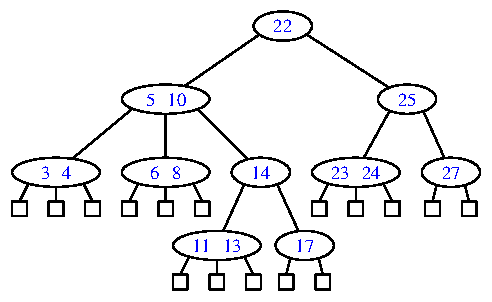
\includegraphics[width=6cm]{asp-11-pic27.pdf}
  \end{center}
\end{frame}

\begin{frame}[fragile]
  \frametitle{Pretraga u n-arnom stablu}
  \begin{itemize}
    \item tražimo ključ $k$ polazeći od korena
    \item u čvoru $w$ poredimo $k$ sa ključevima $k_1, \ldots, k_{d-1}$
    \begin{itemize}
      \item ako je $k=k_i$ za neko $1\leq i\leq d-1$ pronašli smo ključ
      \item inače nastavljamo pretragu od deteta $c_i$ tako da je $k_{i-1}<k<k_i$ 
    \end{itemize}
    \item ako smo došli do lista pretraga je neuspešna
    \item primer: tražimo $k=12$ (neuspešna)
  \end{itemize}
  \begin{center}
    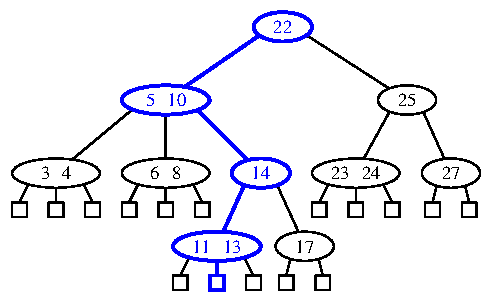
\includegraphics[width=6cm]{asp-11-pic28.pdf}
  \end{center}
\end{frame}

\begin{frame}[fragile]
  \frametitle{Pretraga u n-arnom stablu}
  \begin{itemize}
    \item primer: tražimo $k=24$ (uspešna)
  \end{itemize}
  \begin{center}
    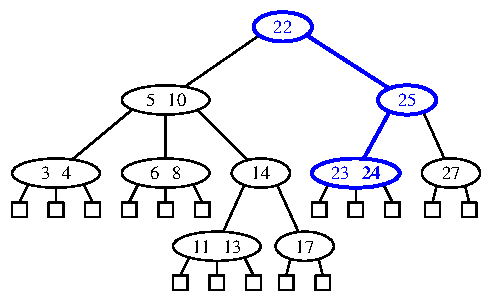
\includegraphics[width=6cm]{asp-11-pic29.pdf}
  \end{center}
\end{frame}

\begin{frame}[fragile]
  \frametitle{Pretraga u n-arnom stablu}
  \begin{itemize}
    \item pretraga unutar čvora?
    \item treba nam \textbf{sekundarna struktura podataka}
    \begin{itemize}
      \item binarna pretraga po nizu je $O(\log d)$
      \item sortirana mapa
    \end{itemize}
    \item pretraga u stablu je $O(h\log d_{\max})$
  \end{itemize}
\end{frame}

\begin{frame}[fragile]
  \frametitle{(2,4) stablo}
  \begin{itemize}
    \item \myred{(2,4) stablo} je n-arno stablo sa dve osobine
    \begin{itemize}
      \item unutrašnji čvor ima najviše 4 deteta
      \item svi listovi imaju istu dubinu
    \end{itemize}
  \end{itemize}
  \begin{center}
    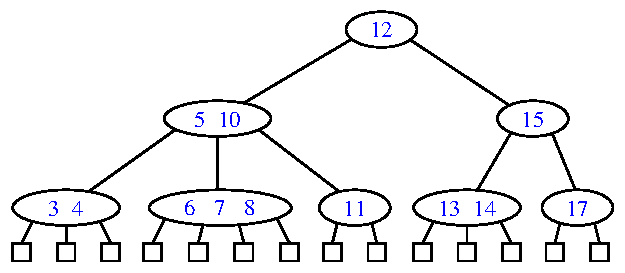
\includegraphics[width=7cm]{asp-11-pic30.pdf}
  \end{center}
  \begin{itemize}
    \item svaki čvor ima 2, 3 ili 4 deteta
    \item visina stabla od $n$ elemenata je $O(\log n)$ 
  \end{itemize}
\end{frame}

\begin{frame}[fragile]
  \frametitle{(2,4) stablo: dodavanje}
  \begin{itemize}
    \item prvo tražimo ključ $k$
    \item neuspešna pretraga se završava u listu
    \item dodamo $k$ u roditelja $w$ tog lista 
    \item (\myred{prelivanje}, \textbf{overflow}): ako je taj roditelj bio 4-čvor, sada je 5-čvor; moramo ga podeliti (\textbf{split}):
  \end{itemize}
  \begin{center}
    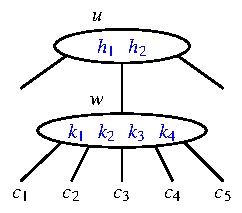
\includegraphics[width=4cm]{asp-11-pic31.pdf}
  \end{center}
\end{frame}

\begin{frame}[fragile]
  \frametitle{(2,4) stablo: dodavanje}
  \begin{itemize}
    \item podela čvora $w$ prilikom prelivanja na $w'$ i $w''$
    \item $w'$ je 3-čvor sa decom $c_1, c_2, c_3$ i ključevima $k_1, k_2$
    \item $w''$ je 2-čvor sa decom $c_4, c_5$ i ključem $k_4$
    \item ključ $k_3$ se penje u roditelja od $w$; ako je $w$ koren, napravi novi čvor 
  \end{itemize}
  \begin{columns}
    \begin{column}[c]{4cm}
      \begin{center}
        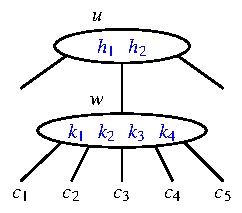
\includegraphics[width=4cm]{asp-11-pic31.pdf}
      \end{center}
    \end{column}
    \begin{column}[c]{4cm}
      \begin{center}
        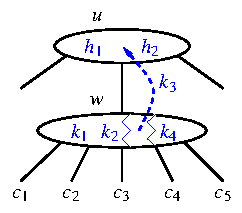
\includegraphics[width=4cm]{asp-11-pic32.pdf}
      \end{center}
    \end{column}
    \begin{column}[c]{4cm}
      \begin{center}
        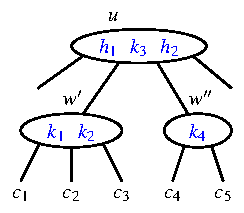
\includegraphics[width=4cm]{asp-11-pic33.pdf}
      \end{center}
    \end{column}
  \end{columns}
  podela može biti kaskadna!
\end{frame}

\begin{frame}[fragile]
  \frametitle{(2,4) stablo: uklanjanje}
  \begin{itemize}
    \item prvi slučaj: uklanjanjem ključa ne narušavaju se osobine (2,4) stabla
    \item primer: uklanjamo 13
  \end{itemize}
  \begin{columns}
    \begin{column}[c]{6cm}
      \begin{center}
        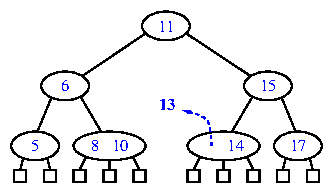
\includegraphics[width=4cm]{asp-11-pic34a.pdf}
      \end{center}
    \end{column}
    \begin{column}[c]{6cm}
      \begin{center}
        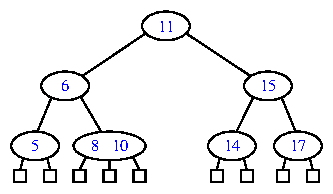
\includegraphics[width=4cm]{asp-11-pic34b.pdf}
      \end{center}
    \end{column}
  \end{columns}
\end{frame}

\begin{frame}[fragile]
  \frametitle{(2,4) stablo: uklanjanje}
  \begin{itemize}
    \item drugi slučaj: uklanjanje iz $w$ izaziva \textbf{underflow}
    \item da li je jedan od najbliže braće 3-čvor ili 4-čvor?
    \item radimo \textbf{transfer}:
    \begin{itemize}
      \item premeštamo ključ iz brata u roditelja
      \item ključ iz roditelja u $w$
    \end{itemize}
    \item primer: uklanjamo 4
  \end{itemize}
  \begin{columns}
    \begin{column}[c]{4cm}
      \begin{center}
        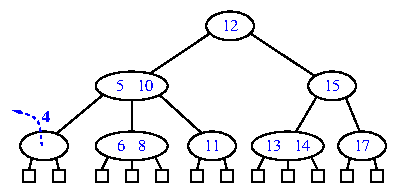
\includegraphics[width=4cm]{asp-11-pic35a.pdf}
      \\ uklanjamo 4
      \end{center}
    \end{column}
    \begin{column}[c]{4cm}
      \begin{center}
        \includegraphics[width=4cm]{asp-11-pic35b.pdf}
      \\ transfer
      \end{center}
    \end{column}
    \begin{column}[c]{4cm}
      \begin{center}
        \includegraphics[width=4cm]{asp-11-pic35c.pdf}
      \\ rezultat
      \end{center}
    \end{column}
  \end{columns}
\end{frame}

\begin{frame}[fragile]
  \frametitle{(2,4) stablo: uklanjanje}
  \begin{itemize}
    \item treći slučaj: uklanjanje izaziva \textbf{underflow}
    \item nijedan od najbliže braće nije 3-čvor ili 4-čvor
    \item radimo \textbf{fuziju}:
    \begin{itemize}
      \item spajamo $w$ sa bratom
      \item ključ iz roditelja spuštamo u spojeni čvor 
    \end{itemize}
    \item primer: uklanjamo 12
  \end{itemize}
  \begin{columns}
    \begin{column}[c]{4cm}
      \begin{center}
        \includegraphics[width=4cm]{asp-11-pic36a.pdf}
      \\ uklanjamo 12
      \end{center}
    \end{column}
    \begin{column}[c]{4cm}
      \begin{center}
        \includegraphics[width=4cm]{asp-11-pic36b.pdf}
      \\ fuzija
      \end{center}
    \end{column}
    \begin{column}[c]{4cm}
      \begin{center}
        \includegraphics[width=4cm]{asp-11-pic36c.pdf}
      \\ rezultat
      \end{center}
    \end{column}
  \end{columns}
\end{frame}

\begin{frame}[fragile]
  \frametitle{(2,4) stablo: uklanjanje}
  \begin{itemize}
    \item fuzija može da propagira underflow
    \item ako se koren isprazni fuzijom, prosto se obriše
  \end{itemize}
  \begin{columns}
    \begin{column}[t]{6cm}
      \begin{center}
        \includegraphics[width=4cm]{asp-11-pic37a.pdf} \\
        \includegraphics[width=4cm]{asp-11-pic37c.pdf}
      \end{center}
    \end{column}
    \begin{column}[t]{6cm}
      \begin{center}
        \includegraphics[width=4cm]{asp-11-pic37b.pdf} \\
        \includegraphics[width=4cm]{asp-11-pic37d.pdf}
      \end{center}
    \end{column}
  \end{columns}
\end{frame}

\begin{frame}[fragile]
  \frametitle{(2,4) stablo: primer dodavanja}
  \begin{itemize}
    \item \textbf{\myred{53}}, 97, 50, 48, 83, 69, 64, 80, 73, 87, 71, 84, 65, 44, 18, 88
    \item stablo je inicijalno prazno, kreiramo koren i dodajemo prvi ključ u njega
  \end{itemize}
  \begin{center}
  \begin{tikzpicture}
  \tikzstyle{bplus}=[rectangle split, rectangle split horizontal,rectangle split ignore empty parts,draw]
  \tikzstyle{every node}=[bplus]
  \tikzstyle{level 1}=[sibling distance=60mm]
  \tikzstyle{level 2}=[sibling distance=15mm]
  \node {53} [->]
  ;\end{tikzpicture}
  \end{center}
\end{frame}
  
\begin{frame}[fragile]
  \frametitle{(2,4) stablo: primer dodavanja}
  \begin{itemize}
    \item 53, \textbf{\myred{97}}, 50, 48, 83, 69, 64, 80, 73, 87, 71, 84, 65, 44, 18, 88
    \item 97 dodajemo u koren, ima mesta
  \end{itemize}
  \begin{center}
  \begin{tikzpicture}
  \tikzstyle{bplus}=[rectangle split, rectangle split horizontal,rectangle split ignore empty parts,draw]
  \tikzstyle{every node}=[bplus]
  \tikzstyle{level 1}=[sibling distance=60mm]
  \tikzstyle{level 2}=[sibling distance=15mm]
  \node {53 \nodepart{two} 97} [->]
  ;\end{tikzpicture}
  \end{center}
\end{frame}
  
\begin{frame}[fragile]
  \frametitle{(2,4) stablo: primer dodavanja}
  \begin{itemize}
    \item 53, 97, \textbf{\myred{50}}, 48, 83, 69, 64, 80, 73, 87, 71, 84, 65, 44, 18, 88
    \item 50 dodajemo u koren, ima mesta
  \end{itemize}
  \begin{center}
  \begin{tikzpicture}
  \tikzstyle{bplus}=[rectangle split, rectangle split horizontal,rectangle split ignore empty parts,draw]
  \tikzstyle{every node}=[bplus]
  \tikzstyle{level 1}=[sibling distance=60mm]
  \tikzstyle{level 2}=[sibling distance=15mm]
  \node {50 \nodepart{two} 53 \nodepart{three} 97} [->]
  ;\end{tikzpicture}
  \end{center}
\end{frame}

\begin{frame}[fragile]
  \frametitle{(2,4) stablo: primer dodavanja}
  \begin{itemize}
    \item 53, 97, 50, \textbf{\myred{48}}, 83, 69, 64, 80, 73, 87, 71, 84, 65, 44, 18, 88
    \item 48 dodajemo u koren, imamo prelivanje
  \end{itemize}
  \begin{tikzpicture}
  \tikzstyle{bplus}=[rectangle split, rectangle split horizontal,rectangle split ignore empty parts,draw]
  \tikzstyle{every node}=[bplus]
  \tikzstyle{level 1}=[sibling distance=60mm]
  \tikzstyle{level 2}=[sibling distance=15mm]
  \node {48 \nodepart{two} 50 \nodepart{three} \myred{53} \nodepart{four} 97} [->]
  ;\end{tikzpicture}
  {\Huge$\Rightarrow$}
  \begin{tikzpicture}
  \tikzstyle{bplus}=[rectangle split, rectangle split horizontal,rectangle split ignore empty parts,draw]
  \tikzstyle{every node}=[bplus]
  \tikzstyle{level 1}=[sibling distance=30mm]
  \tikzstyle{level 2}=[sibling distance=15mm]
  \node {53} [->]
    child {node {48 \nodepart{two} 50}} 
    child {node {97}}
  ;\end{tikzpicture}
  \end{frame}

\begin{frame}[fragile]
  \frametitle{(2,4) stablo: primer dodavanja}
  \begin{itemize}
    \item 53, 97, 50, 48, \textbf{\myred{83}}, 69, 64, 80, 73, 87, 71, 84, 65, 44, 18, 88
    \item nakon prelivanja dodajemo 83, ima mesta
  \end{itemize}
  \begin{center}
  \begin{tikzpicture}
  \tikzstyle{bplus}=[rectangle split, rectangle split horizontal,rectangle split ignore empty parts,draw]
  \tikzstyle{every node}=[bplus]
  \tikzstyle{level 1}=[sibling distance=30mm]
  \tikzstyle{level 2}=[sibling distance=15mm]
  \node {53} [->]
    child {node {48 \nodepart{two} 50}} 
    child {node {83 \nodepart{two} 97}}
  ;\end{tikzpicture}
  \end{center}
\end{frame}

\begin{frame}[fragile]
  \frametitle{(2,4) stablo: primer dodavanja}
  \begin{itemize}
    \item 53, 97, 50, 48, 83, \textbf{\myred{69}}, 64, 80, 73, 87, 71, 84, 65, 44, 18, 88
    \item dodajemo 69, ima mesta
  \end{itemize}
  \begin{center}
  \begin{tikzpicture}
  \tikzstyle{bplus}=[rectangle split, rectangle split horizontal,rectangle split ignore empty parts,draw]
  \tikzstyle{every node}=[bplus]
  \tikzstyle{level 1}=[sibling distance=30mm]
  \tikzstyle{level 2}=[sibling distance=15mm]
  \node {53} [->]
    child {node {48 \nodepart{two} 50}} 
    child {node {69 \nodepart{two} 83 \nodepart{three} 97}}
  ;\end{tikzpicture}
  \end{center}
\end{frame}

\begin{frame}[fragile]
  \frametitle{(2,4) stablo: primer dodavanja}
  \begin{itemize}
    \item 53, 97, 50, 48, 83, 69, \textbf{\myred{64}}, 80, 73, 87, 71, 84, 65, 44, 18, 88
    \item dodajemo 64, imamo prelivanje, 83 se penje u roditelja
  \end{itemize}
  \begin{center}
  \begin{tikzpicture}
  \tikzstyle{bplus}=[rectangle split, rectangle split horizontal,rectangle split ignore empty parts,draw]
  \tikzstyle{every node}=[bplus]
  \tikzstyle{level 1}=[sibling distance=30mm]
  \tikzstyle{level 2}=[sibling distance=15mm]
  \node {53} [->]
    child {node {48 \nodepart{two} 50}} 
    child {node {64 \nodepart{two} 69 \nodepart{three} \myred{83} \nodepart{four} 97}}
  ;\end{tikzpicture}

  {\Huge$\Downarrow$}
  
  \begin{tikzpicture}
    \tikzstyle{bplus}=[rectangle split, rectangle split horizontal,rectangle split ignore empty parts,draw]
    \tikzstyle{every node}=[bplus]
    \tikzstyle{level 1}=[sibling distance=30mm]
    \tikzstyle{level 2}=[sibling distance=15mm]
    \node {53 \nodepart{two} 83} [->]
      child {node {48 \nodepart{two} 50}} 
      child {node {64 \nodepart{two} 69}}
      child {node {97}}
  ;\end{tikzpicture}
  \end{center}
\end{frame}

\begin{frame}[fragile]
  \frametitle{(2,4) stablo: primer dodavanja}
  \begin{itemize}
    \item 53, 97, 50, 48, 83, 69, 64, \textbf{\myred{80}}, 73, 87, 71, 84, 65, 44, 18, 88
    \item dodajemo 80, ima mesta
  \end{itemize}
  \begin{center}
  \begin{tikzpicture}
    \tikzstyle{bplus}=[rectangle split, rectangle split horizontal,rectangle split ignore empty parts,draw]
    \tikzstyle{every node}=[bplus]
    \tikzstyle{level 1}=[sibling distance=30mm]
    \tikzstyle{level 2}=[sibling distance=15mm]
    \node {53 \nodepart{two} 83} [->]
      child {node {48 \nodepart{two} 50}} 
      child {node {64 \nodepart{two} 69 \nodepart{three} 80}}
      child {node {97}}
  ;\end{tikzpicture}
  \end{center}
\end{frame}

\begin{frame}[fragile]
  \frametitle{(2,4) stablo: primer dodavanja}
  \begin{itemize}
    \item 53, 97, 50, 48, 83, 69, 64, 80, \textbf{\myred{73}}, 87, 71, 84, 65, 44, 18, 88
    \item dodajemo 73, imamo prelivanje, 73 se penje u roditelja, tamo ima mesta
  \end{itemize}
  \begin{center}
  \begin{tikzpicture}
    \tikzstyle{bplus}=[rectangle split, rectangle split horizontal,rectangle split ignore empty parts,draw]
    \tikzstyle{every node}=[bplus]
    \tikzstyle{level 1}=[sibling distance=30mm]
    \tikzstyle{level 2}=[sibling distance=15mm]
    \node {53 \nodepart{two} 83} [->]
      child {node {48 \nodepart{two} 50}} 
      child {node {64 \nodepart{two} 69 \nodepart{three} \myred{73} \nodepart{four}80}}
      child {node {97}}
  ;\end{tikzpicture}

  {\Huge$\Downarrow$}

  \begin{tikzpicture}
    \tikzstyle{bplus}=[rectangle split, rectangle split horizontal,rectangle split ignore empty parts,draw]
    \tikzstyle{every node}=[bplus]
    \tikzstyle{level 1}=[sibling distance=20mm]
    \tikzstyle{level 2}=[sibling distance=15mm]
    \node {53 \nodepart{two} 73 \nodepart{three} 83} [->]
      child {node {48 \nodepart{two} 50}} 
      child {node {64 \nodepart{two} 69}}
      child {node {80}}
      child {node {97}}
  ;\end{tikzpicture}
  \end{center}
\end{frame}

\begin{frame}[fragile]
  \frametitle{(2,4) stablo: primer dodavanja}
  \begin{itemize}
    \item 53, 97, 50, 48, 83, 69, 64, 80, 73, \textbf{\myred{87}}, 71, 84, 65, 44, 18, 88
    \item dodajemo 87, ima mesta
  \end{itemize}
  \begin{center}
  \begin{tikzpicture}
    \tikzstyle{bplus}=[rectangle split, rectangle split horizontal,rectangle split ignore empty parts,draw]
    \tikzstyle{every node}=[bplus]
    \tikzstyle{level 1}=[sibling distance=20mm]
    \tikzstyle{level 2}=[sibling distance=15mm]
    \node {53 \nodepart{two} 73 \nodepart{three} 83} [->]
      child {node {48 \nodepart{two} 50}} 
      child {node {64 \nodepart{two} 69}}
      child {node {80}}
      child {node {87 \nodepart{two} 97}}
  ;\end{tikzpicture}
  \end{center}
\end{frame}

\begin{frame}[fragile]
  \frametitle{(2,4) stablo: primer dodavanja}
  \begin{itemize}
    \item 53, 97, 50, 48, 83, 69, 64, 80, 73, 87, \textbf{\myred{71}}, 84, 65, 44, 18, 88
    \item dodajemo 71, ima mesta
  \end{itemize}
  \begin{center}
  \begin{tikzpicture}
    \tikzstyle{bplus}=[rectangle split, rectangle split horizontal,rectangle split ignore empty parts,draw]
    \tikzstyle{every node}=[bplus]
    \tikzstyle{level 1}=[sibling distance=30mm]
    \tikzstyle{level 2}=[sibling distance=15mm]
    \node {53 \nodepart{two} 73 \nodepart{three} 83} [->]
      child {node {48 \nodepart{two} 50}} 
      child {node {64 \nodepart{two} 69 \nodepart{three} 71}}
      child {node {80}}
      child {node {87 \nodepart{two} 97}}
  ;\end{tikzpicture}
\end{center}
\end{frame}

\begin{frame}[fragile]
  \frametitle{(2,4) stablo: primer dodavanja}
  \begin{itemize}
    \item 53, 97, 50, 48, 83, 69, 64, 80, 73, 87, 71, \textbf{\myred{84}}, 65, 44, 18, 88
    \item dodajemo 84, ima mesta
  \end{itemize}
  \begin{center}
  \begin{tikzpicture}
    \tikzstyle{bplus}=[rectangle split, rectangle split horizontal,rectangle split ignore empty parts,draw]
    \tikzstyle{every node}=[bplus]
    \tikzstyle{level 1}=[sibling distance=30mm]
    \tikzstyle{level 2}=[sibling distance=15mm]
    \node {53 \nodepart{two} 73 \nodepart{three} 83} [->]
      child {node {48 \nodepart{two} 50}} 
      child {node {64 \nodepart{two} 69 \nodepart{three} 71}}
      child {node {80}}
      child {node {84 \nodepart{two} 87 \nodepart{three} 97}}
  ;\end{tikzpicture}
\end{center}
\end{frame}

\begin{frame}[fragile]
  \frametitle{(2,4) stablo: primer dodavanja}
  \begin{itemize}
    \item 53, 97, 50, 48, 83, 69, 64, 80, 73, 87, 71, 84, \textbf{\myred{65}}, 44, 18, 88
    \item dodajemo 65, imamo prelivanje, 69 penjemo u roditelja
  \end{itemize}
  \begin{center}
  \begin{tikzpicture}
    \tikzstyle{bplus}=[rectangle split, rectangle split horizontal,rectangle split ignore empty parts,draw]
    \tikzstyle{every node}=[bplus]
    \tikzstyle{level 1}=[sibling distance=30mm]
    \tikzstyle{level 2}=[sibling distance=15mm]
    \node {53 \nodepart{two} 73 \nodepart{three} 83} [->]
      child {node {48 \nodepart{two} 50}} 
      child {node {64 \nodepart{two} 65 \nodepart{three} \myred{69} \nodepart{four} 71}}
      child {node {80}}
      child {node {84 \nodepart{two} 87 \nodepart{three} 97}}
  ;\end{tikzpicture}

  {\Huge$\Downarrow$}

  \begin{tikzpicture}
    \tikzstyle{bplus}=[rectangle split, rectangle split horizontal,rectangle split ignore empty parts,draw]
    \tikzstyle{every node}=[bplus]
    \tikzstyle{level 1}=[sibling distance=20mm]
    \tikzstyle{level 2}=[sibling distance=15mm]
    \node {53 \nodepart{two} 69 \nodepart{three} 73 \nodepart{four} 83} [->]
      child {node {48 \nodepart{two} 50}} 
      child {node {64 \nodepart{two} 65}}
      child {node {71}}
      child {node {80}}
      child {node {84 \nodepart{two} 87 \nodepart{three} 97}}
  ;\end{tikzpicture}
\end{center}
\end{frame}

\begin{frame}[fragile]
  \frametitle{(2,4) stablo: primer dodavanja}
  \begin{itemize}
    \item 53, 97, 50, 48, 83, 69, 64, 80, 73, 87, 71, 84, \textbf{\myred{65}}, 44, 18, 88
    \item sada u korenu imamo prelivanje i pravimo novi koren
  \end{itemize}
  \begin{center}
    \begin{tikzpicture}
      \tikzstyle{bplus}=[rectangle split, rectangle split horizontal,rectangle split ignore empty parts,draw]
      \tikzstyle{every node}=[bplus]
      \tikzstyle{level 1}=[sibling distance=20mm,level distance=10mm]
      \tikzstyle{level 2}=[sibling distance=15mm,level distance=10mm]
      \node {53 \nodepart{two} 69 \nodepart{three} \myred{73} \nodepart{four} 83} [->]
        child {node {48 \nodepart{two} 50}} 
        child {node {64 \nodepart{two} 65}}
        child {node {71}}
        child {node {80}}
        child {node {84 \nodepart{two} 87 \nodepart{three} 97}}
    ;\end{tikzpicture}
  
    {\Large$\Downarrow$}

    \begin{tikzpicture}
      \tikzstyle{bplus}=[rectangle split, rectangle split horizontal,rectangle split ignore empty parts,draw]
      \tikzstyle{every node}=[bplus]
      \tikzstyle{level 1}=[sibling distance=40mm,level distance=10mm]
      \tikzstyle{level 2}=[sibling distance=15mm,level distance=10mm]
      \node {73} [->]
        child {node {53 \nodepart{two} 69}
          child {node {48 \nodepart{two} 50}} 
          child {node {64 \nodepart{two} 65}}
          child {node {71}}
        }
        child {node{83}
          child {node {80}}
          child {node {84 \nodepart{two} 87 \nodepart{three} 97}}
        }
    ;\end{tikzpicture}
  \end{center}
\end{frame}

\begin{frame}[fragile]
  \frametitle{(2,4) stablo: primer dodavanja}
  \begin{itemize}
    \item (2,4) stablo povećava broj nivoa kada se desi prelivanje u korenu
    \item raste ,,iz korena`` umesto ,,kroz listove``
    \item u prethodnom koraku je 73 postao novi koren nakon prelivanja
  \end{itemize}
  \begin{center}
    \begin{tikzpicture}
      \tikzstyle{bplus}=[rectangle split, rectangle split horizontal,rectangle split ignore empty parts,draw]
      \tikzstyle{every node}=[bplus]
      \tikzstyle{level 1}=[sibling distance=40mm]
      \tikzstyle{level 2}=[sibling distance=15mm]
      \node {73} [->]
        child {node {53 \nodepart{two} 69}
          child {node {48 \nodepart{two} 50}} 
          child {node {64 \nodepart{two} 65}}
          child {node {71}}
        }
        child {node{83}
          child {node {80}}
          child {node {84 \nodepart{two} 87 \nodepart{three} 97}}
        }
    ;\end{tikzpicture}
  \end{center}
\end{frame}

\begin{frame}[fragile]
  \frametitle{(2,4) stablo: primer dodavanja}
  \begin{itemize}
    \item 53, 97, 50, 48, 83, 69, 64, 80, 73, 87, 71, 84, 65, \textbf{\myred{44}}, 18, 88
    \item dodajemo 44, ima mesta
  \end{itemize}
  \begin{center}
    \begin{tikzpicture}
      \tikzstyle{bplus}=[rectangle split, rectangle split horizontal,rectangle split ignore empty parts,draw]
      \tikzstyle{every node}=[bplus]
      \tikzstyle{level 1}=[sibling distance=40mm]
      \tikzstyle{level 2}=[sibling distance=20mm]
      \node {73} [->]
        child {node {53 \nodepart{two} 69}
          child {node {44 \nodepart{two} 48 \nodepart{three} 50}} 
          child {node {64 \nodepart{two} 65}}
          child {node {71}}
        }
        child {node{83}
          child {node {80}}
          child {node {84 \nodepart{two} 87 \nodepart{three} 97}}
        }
    ;\end{tikzpicture}
  \end{center}
\end{frame}

\begin{frame}[fragile]
  \frametitle{(2,4) stablo: primer dodavanja}
  \begin{itemize}
    \item 53, 97, 50, 48, 83, 69, 64, 80, 73, 87, 71, 84, 65, 44, \textbf{\myred{18}}, 88
    \item dodajemo 18, imamo prelivanje, 48 ide u roditelja
  \end{itemize}
  \begin{center}
    \begin{tikzpicture}
      \tikzstyle{bplus}=[rectangle split, rectangle split horizontal,rectangle split ignore empty parts,draw]
      \tikzstyle{every node}=[bplus]
      \tikzstyle{level 1}=[sibling distance=50mm]
      \tikzstyle{level 2}=[sibling distance=25mm]
      \node {73} [->]
        child {node {53 \nodepart{two} 69}
          child {node {18 \nodepart{two} 44 \nodepart{three} \myred{48} \nodepart{four} 50}} 
          child {node {64 \nodepart{two} 65}}
          child {node {71}}
        }
        child {node{83}
          child {node {80}}
          child {node {84 \nodepart{two} 87 \nodepart{three} 97}}
        }
    ;\end{tikzpicture}
  \end{center}
\end{frame}

\begin{frame}[fragile]
  \frametitle{(2,4) stablo: primer dodavanja}
  \begin{itemize}
    \item 53, 97, 50, 48, 83, 69, 64, 80, 73, 87, 71, 84, 65, 44, \textbf{\myred{18}}, 88
    \item nakon prelivanja
  \end{itemize}
  \begin{center}
    \begin{tikzpicture}
      \tikzstyle{bplus}=[rectangle split, rectangle split horizontal,rectangle split ignore empty parts,draw]
      \tikzstyle{every node}=[bplus]
      \tikzstyle{level 1}=[sibling distance=40mm]
      \tikzstyle{level 2}=[sibling distance=15mm]
      \node {73} [->]
        child {node {48 \nodepart{two} 53 \nodepart{three} 69}
          child {node {18 \nodepart{two} 44}}
          child {node {50}} 
          child {node {64 \nodepart{two} 65}}
          child {node {71}}
        }
        child {node{83}
          child {node {80}}
          child {node {84 \nodepart{two} 87 \nodepart{three} 97}}
        }
    ;\end{tikzpicture}
  \end{center}
\end{frame}

\begin{frame}[fragile]
  \frametitle{(2,4) stablo: primer dodavanja}
  \begin{itemize}
    \item 53, 97, 50, 48, 83, 69, 64, 80, 73, 87, 71, 84, 65, 44, 18, \textbf{\myred{88}}
    \item dodajemo 88, imamo prelivanje, 88 ide u roditelja
  \end{itemize}
  \begin{center}
    \begin{tikzpicture}
      \tikzstyle{bplus}=[rectangle split, rectangle split horizontal,rectangle split ignore empty parts,draw]
      \tikzstyle{every node}=[bplus]
      \tikzstyle{level 1}=[sibling distance=50mm]
      \tikzstyle{level 2}=[sibling distance=20mm]
      \node {73} [->]
        child {node {48 \nodepart{two} 53 \nodepart{three} 69}
          child {node {18 \nodepart{two} 44}}
          child {node {50}} 
          child {node {64 \nodepart{two} 65}}
          child {node {71}}
        }
        child {node{83}
          child {node {80}}
          child {node {84 \nodepart{two} 87 \nodepart{three} \myred{88} \nodepart{four} 97}}
        }
    ;\end{tikzpicture}
  \end{center}
\end{frame}

\begin{frame}[fragile]
  \frametitle{(2,4) stablo: primer dodavanja}
  \begin{itemize}
    \item 53, 97, 50, 48, 83, 69, 64, 80, 73, 87, 71, 84, 65, 44, 18, \textbf{\myred{88}}
    \item nakon prelivanja
  \end{itemize}
  \begin{center}
    \begin{tikzpicture}
      \tikzstyle{bplus}=[rectangle split, rectangle split horizontal,rectangle split ignore empty parts,draw]
      \tikzstyle{every node}=[bplus]
      \tikzstyle{level 1}=[sibling distance=50mm]
      \tikzstyle{level 2}=[sibling distance=15mm]
      \node {73} [->]
        child {node {48 \nodepart{two} 53 \nodepart{three} 69}
          child {node {18 \nodepart{two} 44}}
          child {node {50}} 
          child {node {64 \nodepart{two} 65}}
          child {node {71}}
        }
        child {node{83 \nodepart{two} 88}
          child {node {80}}
          child {node {84 \nodepart{two} 87}}
          child {node {97}}
        }
    ;\end{tikzpicture}
  \end{center}
\end{frame}

\begin{frame}[fragile]
  \frametitle{(2,4) stablo: performanse}
  \begin{itemize}
    \item \textbf{dodavanje} u (2,4) stablu sa $n$ elemenata
    \begin{itemize}
      \item visina stabla je $O(\log n)$
      \item traženje ključa je $O(\log n)$
      \item dodavanje novog ključa u čvor je $O(1)$
      \item svaka podela čvora je $O(1)$
      \item ukupan broj podela je $O(\log n)$ \\ \ \\
    \end{itemize}
    \item $\Rightarrow$ dodavanje je $O(\log n)$ 
  \end{itemize}
\end{frame}

\begin{frame}[fragile]
  \frametitle{(2,4) stablo: performanse}
  \begin{itemize}
    \item \textbf{uklanjanje} u (2,4) stablu sa $n$ elemenata
    \begin{itemize}
      \item visina stabla je $O(\log n)$
      \item traženje ključa je $O(\log n)$
      \item uklanjanje ključa je $O(1)$
      \item može da usledi $O(\log n)$ iza kojih je max 1 transfer
      \item fuzija i transfer su $O(1)$ \\ \ \\
    \end{itemize}
    \item $\Rightarrow$ uklanjanje je $O(\log n)$ 
  \end{itemize}
\end{frame}

\begin{frame}[fragile]
  \frametitle{Različite implementacije mape}
  \begin{tabular}{p{2cm}|p{1cm}|p{1cm}|p{1cm}|p{6cm}}
  & \textbf{search} & \textbf{insert} & \textbf{delete} & \textbf{napomene} \\ \hline\hline
  hash tabela & 1 \mbox{\tiny očekivano} & 1 \mbox{\tiny očekivano} & 1 \mbox{\tiny očekivano} & {\scriptsize nema metode za sortiranu mapu; jednostavna implementacija} \\ \hline
  skip lista & $\log n$ \mbox{\tiny verovatno} & $\log n$ \mbox{\tiny verovatno} & $\log n$ \mbox{\tiny verovatno} & {\scriptsize randomized insert; jednostavna implementacija} \\ \hline
  AVL i (2,4) & $\log n$ \mbox{\tiny najgore} & $\log n$ \mbox{\tiny najgore} & $\log n$ \mbox{\tiny najgore} & {\scriptsize komplikovana implementacija} \\ \hline
  \end{tabular}
\end{frame}

\section[RB stablo]{Crveno-crno stablo}

\begin{frame}[fragile]
  \frametitle{Crveno-crno stablo}
  \begin{itemize}
    \item \textbf{\myred{red}-black} stablo je reprezentacija (2,4) stabla pomoću binarnog stabla čiji čvorovi su obojeni \textbf{\myred{crveno}} ili \textbf{crno}
    \item u poređenju sa (2,4) stablom, RB stablo ima
    \begin{itemize}
      \item jednake $O(\log n)$ performanse
      \item jednostavniju implementaciju
    \end{itemize}
  \end{itemize}
\end{frame}

\begin{frame}[fragile]
  \frametitle{(2,4) stablo i crveno-crno stablo}
  \begin{center}
    \includegraphics[width=7cm]{asp-11-pic30.pdf} \\
    \includegraphics[width=7cm]{asp-11-pic38.pdf}
  \end{center}
\end{frame}

\begin{frame}[fragile]
  \frametitle{Crveno-crno stablo: definicija}
  \begin{itemize}
    \item \myred{crveno-}crno stablo je binarno stablo pretrage sa osobinama
    \begin{itemize}
      \item koren je \textbf{crn}
      \item deca \textbf{\myred{crvenog}} čvora su \textbf{crna}
      \begin{itemize}
        \item deca \textbf{crnog} čvora ne moraju biti \textbf{\myred{crvena}}!
      \end{itemize}
      \item sve putanje od korena do lista sadrže isti broj \textbf{crnih} čvorova
      \begin{itemize}
        \item \textbf{crna dubina} čvora: broj crnih predaka (računajući i dati čvor)
      \end{itemize}
    \end{itemize}
  \end{itemize}
\end{frame}

\begin{frame}[fragile]
  \frametitle{Crveno-crno stablo: posledice}
  \begin{itemize}
    \item putanja od korena do najdaljeg lista nije više od duplo duža od putanje do najbližeg lista
    \item RB-stablo je \textit{prilično dobro} balansirano
    \item visina RB stabla sa $n$ elemenata je $O(\log n)$
    \item pretraga na isti način kao za binarno stablo
    \item pretraga je takođe $O(\log n)$
  \end{itemize}
\end{frame}

\begin{frame}[fragile]
  \frametitle{Crveno-crno stablo: dodavanje}
  \begin{itemize}
    \item dodavanje na isti način kao za binarno stablo 
    \item novi čvor se boji u \myred{crveno} ako nije koren; koren je uvek crn
      \item ako je roditelj novog čvora crven tada imamo \myred{duplo crveno} -- potrebna je reorganizacija stabla
  \end{itemize}
\end{frame}

\begin{frame}[fragile]
  \frametitle{[add] Korekcija duplog crvenog: stric je crn}
  \begin{itemize}
    \item slučaj 1: brat roditelja novog čvora je crn ili ne postoji
    \item radimo tri-node restructuring
    \item četiri moguće situacije, sa istim rezultatom:
  \end{itemize}
  \begin{center}
    \includegraphics[width=2.5cm]{asp-11-pic39a.pdf}
    \includegraphics[width=2.5cm]{asp-11-pic39b.pdf}
    \includegraphics[width=2.5cm]{asp-11-pic39c.pdf}
    \includegraphics[width=2.5cm]{asp-11-pic39d.pdf} \\
    \includegraphics[width=2.5cm]{asp-11-pic39e.pdf}
  \end{center}
\end{frame}

\begin{frame}[fragile]
  \frametitle{[add] Korekcija duplog crvenog: stric je crven}
  \begin{itemize}
    \item slučaj 2: brat roditelja novog čvora je crven
    \item radimo \textbf{recoloring}:
    \begin{itemize}
      \item obojimo roditelja i strica u crno a dedu u crveno (ako je deda koren, ostaje crn)
    \end{itemize}
    \item moguća propagacija uz stablo
  \end{itemize}
  \includegraphics[width=7cm]{asp-11-pic40a.pdf} \\
  \includegraphics[width=7cm]{asp-11-pic40b.pdf}
\end{frame}

\begin{frame}[fragile]
  \frametitle{[add] Primer: korak 1}
  \begin{itemize}
    \item stablo je na početku prazno
    \item dodajemo 4
    \item on će biti koren
    \item bojimo ga u crno
  \end{itemize}
  \begin{center}
    \includegraphics[scale=1.0]{asp-11-add-01.pdf}
  \end{center}
\end{frame}

\begin{frame}[fragile]
  \frametitle{[add] Primer: korak 2}
  \begin{itemize}
    \item dodajemo 7 kao desno dete od 4
    \item bojimo ga u crveno
    \item nije potrebno restrukturiranje
  \end{itemize}
  \begin{center}
    \includegraphics[scale=1.0]{asp-11-add-02.pdf}
  \end{center}
\end{frame}

\begin{frame}[fragile]
  \frametitle{[add] Primer: korak 3}
  \begin{itemize}
    \item dodajemo 12 kao desno dete od 7
    \item bojimo ga u crveno
    \item imamo duplo crveno
  \end{itemize}
  \begin{center}
    \includegraphics[scale=1.0]{asp-11-add-03.pdf}
  \end{center}
\end{frame}

\begin{frame}[fragile]
  \frametitle{[add] Primer: korak 3a}
  \begin{itemize}
    \item 12 nema strica: slučaj 1
    \item radimo tri-node restructuring
  \end{itemize}
  \begin{center}
    \includegraphics[scale=1.0]{asp-11-add-03.pdf} $\Rightarrow$
    \includegraphics[scale=1.0]{asp-11-add-04.pdf}
  \end{center}
\end{frame}

\begin{frame}[fragile]
  \frametitle{[add] Primer: korak 4}
  \begin{itemize}
    \item dodajemo 15 kao desno dete od 12
    \item bojimo ga u crveno
    \item imamo duplo crveno
  \end{itemize}
  \begin{center}
    \includegraphics[scale=1.0]{asp-11-add-05.pdf}
  \end{center}
\end{frame}

\begin{frame}[fragile]
  \frametitle{[add] Primer: korak 4a}
  \begin{itemize}
    \item 15 ima crvenog strica: slučaj 2
    \item radimo recoloring: obojimo oca i strica u crno a dedu u crveno osim ako je koren
  \end{itemize}
  \begin{center}
    \includegraphics[scale=1.0]{asp-11-add-05.pdf} $\Rightarrow$
    \includegraphics[scale=1.0]{asp-11-add-06.pdf}
  \end{center}
\end{frame}

\begin{frame}[fragile]
  \frametitle{[add] Primer: korak 5}
  \begin{itemize}
    \item dodajemo 3 kao levo dete od 4
    \item bojimo ga u crveno
    \item sve je u redu
  \end{itemize}
  \begin{center}
    \includegraphics[scale=1.0]{asp-11-add-07.pdf}
  \end{center}
\end{frame}

\begin{frame}[fragile]
  \frametitle{[add] Primer: korak 6}
  \begin{itemize}
    \item dodajemo 5 kao desno dete od 4
    \item bojimo ga u crveno
    \item sve je u redu
  \end{itemize}
  \begin{center}
    \includegraphics[scale=1.0]{asp-11-add-08.pdf}
  \end{center}
\end{frame}

\begin{frame}[fragile]
  \frametitle{[add] Primer: korak 7}
  \begin{itemize}
    \item dodajemo 14 kao levo dete od 15
    \item bojimo ga u crveno
    \item imamo duplo crveno
  \end{itemize}
  \begin{center}
    \includegraphics[scale=1.0]{asp-11-add-09.pdf}
  \end{center}
\end{frame}

\begin{frame}[fragile]
  \frametitle{[add] Primer: korak 7a}
  \begin{itemize}
    \item 14 nema strica: slučaj 1
    \item radimo tri-node restructuring za 12-15-14
  \end{itemize}
  \begin{center}
    \includegraphics[scale=1.0]{asp-11-add-09.pdf} $\Rightarrow$
    \includegraphics[scale=1.0]{asp-11-add-10.pdf}
  \end{center}
\end{frame}

\begin{frame}[fragile]
  \frametitle{[add] Primer: korak 8}
  \begin{itemize}
    \item dodajemo 18 kao desno dete od 15
    \item bojimo ga u crveno
    \item imamo duplo crveno
  \end{itemize}
  \begin{center}
    \includegraphics[scale=0.8]{asp-11-add-11.pdf}
  \end{center}
\end{frame}

\begin{frame}[fragile]
  \frametitle{[add] Primer: korak 8a}
  \begin{itemize}
    \item 18 ima crvenog strica: slučaj 2
    \item radimo recoloring: oca i strica u crno a dedu u crveno
  \end{itemize}
  \begin{center}
    \includegraphics[scale=0.8]{asp-11-add-11.pdf} $\Rightarrow$
    \includegraphics[scale=0.8]{asp-11-add-12.pdf}
  \end{center}
\end{frame}

\begin{frame}[fragile]
  \frametitle{[add] Primer: korak 9}
  \begin{itemize}
    \item dodajemo 16 kao levo dete od 18
    \item bojimo ga u crveno
    \item imamo duplo crveno
  \end{itemize}
  \begin{center}
    \includegraphics[scale=0.8]{asp-11-add-13.pdf}
  \end{center}
\end{frame}

\begin{frame}[fragile]
  \frametitle{[add] Primer: korak 9a}
  \begin{itemize}
    \item 16 nema strica: slučaj 1
    \item radimo tri-node restructuring za 15-18-16
  \end{itemize}
  \begin{center}
    \includegraphics[scale=0.8]{asp-11-add-13.pdf} $\Rightarrow$
    \includegraphics[scale=0.8]{asp-11-add-14.pdf}
  \end{center}
\end{frame}

\begin{frame}[fragile]
  \frametitle{[add] Primer: korak 10}
  \begin{itemize}
    \item dodajemo 17 kao levo dete od 18
    \item bojimo ga u crveno
    \item imamo duplo crveno
  \end{itemize}
  \begin{center}
    \includegraphics[scale=0.8]{asp-11-add-15.pdf}
  \end{center}
\end{frame}

\begin{frame}[fragile]
  \frametitle{[add] Primer: korak 10a}
  \begin{itemize}
    \item 17 ima crvenog strica: slučaj 2
    \item radimo recoloring: oca i strica u crno a dedu u crveno
  \end{itemize}
  \begin{center}
    \includegraphics[scale=0.8]{asp-11-add-15.pdf} $\Rightarrow$
    \includegraphics[scale=0.8]{asp-11-add-16.pdf}
  \end{center}
\end{frame}

\begin{frame}[fragile]
  \frametitle{[add] Primer: korak 10b}
  \begin{itemize}
    \item sada je deda (16) u problemu - imamo duplo crveno
    \item 16 ima crnog strica: slučaj 1
    \item radimo tri-node restructuring za 7-14-16
  \end{itemize}
  \begin{center}
    \includegraphics[scale=0.8]{asp-11-add-16.pdf} $\Rightarrow$
    \includegraphics[scale=0.8]{asp-11-add-17.pdf}
  \end{center}
\end{frame}

\begin{frame}[fragile]
  \frametitle{Crveno-crno stablo: uklanjanje}
  \begin{itemize}
    \item uklanjanje na isti način kao za binarno stablo 
    \item $\Rightarrow$ uklanja se čvor koji ima najviše jedno dete
    \item ako je uklonjeni čvor bio crven sve je OK (ne menja se crna dubina)
    \item ako je uklonjeni čvor bio crn:
    \begin{itemize}
      \item ako je uklonjeni čvor list - njegov brat je koren podstabla sa crnom dubinom 1
      \item ako mu je dete crveno: pomeramo dete na mesto uklonjenog roditelja i bojimo crno
      \item ako mu je dete crno: gubimo jedan crni čvor na putanji, narušava se crna dubina u tom podstablu
    \end{itemize}
  \end{itemize}
\end{frame}

\begin{frame}[fragile]
  \frametitle{Korekcija crne dubine}
  \begin{itemize}
    \item uklonjeni crni čvor je bio koren podstabla $T_{\text{light}}$
    \item gledamo šta se nalazi u podstablu njegovog brata $y$ 
    \item (brat mora da postoji jer bi inače bila narušena crna dubina)
  \end{itemize}
  \begin{center}
    \includegraphics[width=5cm]{asp-11-pic41.pdf}
  \end{center}
\end{frame}

\begin{frame}[fragile]
  \frametitle{Korekcija crne dubine 1: brat je crn i ima crveno dete}
  \begin{itemize}
    \item \textbf{slučaj 1}: brat $y$ je crn i ima crveno dete $x$
    \item radimo \textbf{tri-node restructuring}
  \end{itemize}
  \begin{center}
    \includegraphics[width=9cm]{asp-11-pic42a.pdf} \\
    \includegraphics[width=9cm]{asp-11-pic42b.pdf} \\
  \end{center}
  {\scriptsize (druga dva slučaja su simetrična)}
\end{frame}

\begin{frame}[fragile]
  \frametitle{Korekcija crne dubine 2: brat je crn i ima dva crna deteta}  
  \begin{itemize}
    \item \textbf{slučaj 2}: brat $y$ je crn i oba deteta su mu crna ili ih nema
    \item radimo \textbf{recoloring}
    \item ako je $z$ bio crven, tu je kraj; ako je bio crn, recoloring propagira prema gore
  \end{itemize}
  \begin{center}
    \includegraphics[width=8cm]{asp-11-pic43a.pdf} \\
    \includegraphics[width=8cm]{asp-11-pic43b.pdf} \\
  \end{center}
\end{frame}

\begin{frame}[fragile]
  \frametitle{Korekcija crne dubine 3: brat je crven}
  \begin{itemize}
    \item \textbf{slučaj 3}: brat $y$ je crven
    \item radimo \textbf{rotaciju} pa \textbf{recoloring}
    \item čvor $y'$ je crn pa treba primeniti slučaj 1 ili slučaj 2 na njega
  \end{itemize}
  \begin{center}
    \includegraphics[width=8cm]{asp-11-pic44.pdf}
  \end{center}
\end{frame}

\begin{frame}[fragile]
  \frametitle{[remove] Primer: korak 1}
  \begin{itemize}
    \item uklanjamo 3
    \item 3 je crven: ne menja se crna dubina
  \end{itemize}
  \begin{center}
    \includegraphics[scale=0.8]{asp-11-del-01.pdf} $\Rightarrow$
    \includegraphics[scale=0.8]{asp-11-del-02.pdf}
  \end{center}
\end{frame}

\begin{frame}[fragile]
  \frametitle{[remove] Primer: korak 2}
  \begin{itemize}
    \item uklanjamo 12 - to je crni list
    \item njegov brat je crn i ima crveno dete
    \item slučaj 1: radimo tri-node restructuring
  \end{itemize}
  \begin{center}
    \includegraphics[scale=0.8]{asp-11-del-02.pdf} $\Rightarrow$
    \includegraphics[scale=0.8]{asp-11-del-03.pdf}
  \end{center}
\end{frame}

\begin{frame}[fragile]
  \frametitle{[remove] Primer: korak 2a}
  \begin{itemize}
    \item slučaj 1: radimo tri-node restructuring za 7-4-5
  \end{itemize}
  \begin{center}
    \includegraphics[scale=0.8]{asp-11-del-03.pdf} $\Rightarrow$
    \includegraphics[scale=0.8]{asp-11-del-04.pdf}
  \end{center}
\end{frame}

\begin{frame}[fragile]
  \frametitle{[remove] Primer: korak 3}
  \begin{itemize}
    \item uklanjamo 17 - to je crveni list
  \end{itemize}
  \begin{center}
    \includegraphics[scale=0.8]{asp-11-del-04.pdf} $\Rightarrow$
    \includegraphics[scale=0.8]{asp-11-del-05.pdf}
  \end{center}
\end{frame}

\begin{frame}[fragile]
  \frametitle{[remove] Primer: korak 4}
  \begin{itemize}
    \item uklanjamo 18 - crni list
    \item njegov crni brat nema dece
    \item slučaj 2: recoloring - menjamo boju brata i roditelja
  \end{itemize}
  \begin{center}
    \includegraphics[scale=0.8]{asp-11-del-05.pdf} $\Rightarrow$
    \includegraphics[scale=0.8]{asp-11-del-06.pdf}
  \end{center}
\end{frame}

\begin{frame}[fragile]
  \frametitle{[remove] Primer: korak 4a}
  \begin{itemize}
    \item slučaj 2: recoloring - menjamo boju brata i roditelja
  \end{itemize}
  \begin{center}
    \includegraphics[scale=0.8]{asp-11-del-06.pdf} $\Rightarrow$
    \includegraphics[scale=0.8]{asp-11-del-07.pdf}
  \end{center}
\end{frame}

\begin{frame}[fragile]
  \frametitle{[remove] Primer: korak 5}
  \begin{itemize}
    \item uklanjamo 15 - crveni list
  \end{itemize}
  \begin{center}
    \includegraphics[scale=0.8]{asp-11-del-07.pdf} $\Rightarrow$
    \includegraphics[scale=0.8]{asp-11-del-08.pdf}
  \end{center}
\end{frame}

\begin{frame}[fragile]
  \frametitle{[remove] Primer: korak 6}
  \begin{itemize}
    \item uklanjamo 16 - crni list
    \item njegov brat 5 je crven: slučaj 3
  \end{itemize}
  \begin{center}
    \includegraphics[scale=0.8]{asp-11-del-08.pdf}
  \end{center}
\end{frame}

\begin{frame}[fragile]
  \frametitle{[remove] Primer: korak 6a}
  \begin{itemize}
    \item slučaj 3: radimo rotaciju pa recoloring
  \end{itemize}
  \begin{center}
    \includegraphics[scale=0.8]{asp-11-del-09.pdf} $\Rightarrow$
    \includegraphics[scale=0.8]{asp-11-del-10.pdf} $\Rightarrow$
    \includegraphics[scale=0.8]{asp-11-del-11.pdf}
  \end{center}
\end{frame}

\begin{frame}[fragile]
  \frametitle{Crveno-crno stablo: performanse}
  \begin{itemize}
    \item jednake kao i za (2,4) stablo
    \item sve operacije su $O(\log n)$ 
    \item dodavanje i uklanjanje zahtevaju konstantan broj operacija restrukturiranja \\ \ \\
    \item odličan interaktivni demo za RB stabla: \\
    \url{http://gauss.ececs.uc.edu/RedBlack/redblack.html}
  \end{itemize}
\end{frame}

\end{document}
